\documentclass[12pt]{extarticle}

%%%% paramètres généraux et commandes prédéfinies
\input{parametres}
\usepackage{lmodern}

%% Ces commandes sont adaptées du très bon paquet ProfLycée de Cedric Pierquet 
%% https://ctan.org/pkg/proflycee
\tcbset{
  style code Tex/.style = {%
    listing engine = listings,%
    listing options = {%
      breaklines = true,%
      breakatwhitespace = true,%
      style = tcblatex, basicstyle = \footnotesize\ttfamily,%
      tabsize = 2,%
      commentstyle = {\itshape\color{couleurSec-300}},
      keywordstyle = {\color{couleurSec}},%
      classoffset = 0,%
      keywords = {chemfig, definesubmol},%
      alsoletter = {-},%
      keywordstyle = {\color{couleurSec}}%
    }
  },
  cote a cote/.style = {%
    listing side text,%
    righthand width = #1%
  }
}

%% de Cedric Pierquet https://ctan.org/pkg/proflycee
\NewTCBListing{boiteCodeTex}{ O{couleurTer} m }{%
  enhanced, breakable,%
  flush right, boxrule = 1pt, colframe = #1!90,%
  sharp corners, top = 0mm, bottom = 0mm, left = 0.4em, right = 5mm,%
  before skip = \baselineskip, after skip = \baselineskip,%
  colback = white,%
  fontupper = \footnotesize, fontlower = \footnotesize,%
  title = {{\scriptsize\faCogs} Code \LaTeX},%
  fonttitle = \bfseries\footnotesize\sffamily, colbacktitle = #1,%
  style code Tex,%
  #2,%
}


%%%% doc
\begin{document}
  \titre{Biomolécules}
  \begin{center}
    Quelques commandes pour tracer des biomolécules dans le cadre du lycée.
  \end{center}

  \tableofcontents
  \newpage

  \section{Logique interne}

%%
\subsection{Nom des molécules}

Pour tracer une molécule, il suffit d'appeler \lstinline|\chemfig\{!\nomDeLaMolecule}|.
La représentation de base pour les molécules est la formule topologique, il faut ajouter un suffixe au nom pour passer à une autre représentation \important{si elle est définie, ce qui n'est pas du tout toujours le cas.} Les suffixes sont les suivants :

\begin{listePoints}[2]
  \item \lstinline{SemiDev} : formule semi-développée ;
  \item \lstinline{Dev} : formule développée ;
  \item \lstinline{Haw} : représentation de Haworth ;
  \item \lstinline{Cram} : représentation de Cram.
\end{listePoints}
Pour les acides aminés, il existe quatre autres suffixes
\begin{listePoints}[2]
  \item \lstinline{L} : représentation de Fischer gauche ;
  \item \lstinline{H} : pour tracer un polypeptide, la chaîne latérale est vers le haut ;
  \item \lstinline{D} : représentation de Fischer droite ;
  \item \lstinline{B} : pour tracer un polypeptide, la chaîne latérale est vers le bas.
\end{listePoints}

%%
\subsection{Commandes internes pour faciliter l'écriture}

Pour tracer les formules topologiques, 
j'utilise plusieurs commandes pour éviter d'avoir à spécifier en permanence les angles les plus courants
(\qty{60}{\degree}, \qty{50}{\degree}, etc.),
ou pour réutiliser des morceaux de molécules complexes

\begin{boiteCodeTex}{cote a cote = 2cm}
  \chemfig{-!\vide{::30} -} % Pour tracer une liaison invisible (utile pour les cycles incomplets)

  \chemfig{-!\vide{::-30}-}
\end{boiteCodeTex}
%
\begin{boiteCodeTex}{cote a cote = 2cm}
  \chemfig{-[:30] !\lh} % Pour tracer une liaison vers le haut (liaison haut = lh)

  \chemfig{-[:30] !\lb} % Pour tracer une liaison vers le bas (liaison bas = lb)
\end{boiteCodeTex}
%
\begin{boiteCodeTex}{cote a cote = 2cm}
  \chemfig{-[:30]!\lhb} % Pour tracer une liaison vers le haut puis vers le bas

  \chemfig{-[:30]!\lbh} % Pour tracer une liaison vers le bas puis vers le haut
\end{boiteCodeTex}
%
\begin{boiteCodeTex}{cote a cote = 2cm}
  \chemfig{-[:30]!\llh} % Pour tracer une liaison double vers le haut
  
  \chemfig{-[:30]!\llb} % Pour tracer une liaison double vers le bas
\end{boiteCodeTex}
%
\begin{boiteCodeTex}{cote a cote = 3cm}
  \chemfig{-[:-30]!\cis} % Pour tracer une liaison cis
  
  \chemfig{-[:-30]!\trans} % Pour tracer une liaison "trans" aplatie
\end{boiteCodeTex}
%
\begin{boiteCodeTex}{cote a cote = 2cm}
  \chemfig{-[:30]!\ldh} % Pour tracer une liaison développée vers le haut (l'angle est plus faible)
  
  \chemfig{-[:30]!\ldb} % Pour tracer une liaison développée vers le bas
\end{boiteCodeTex}
%
\begin{boiteCodeTex}{cote a cote = 2cm}
  \chemfig{-[:30]!\lldh} % Pour tracer une liaison double développée vers le haut
  
  \chemfig{-[:30]!\lldb} % Pour tracer une liaison double développée vers le bas
\end{boiteCodeTex}
%
\begin{boiteCodeTex}{cote a cote = 2cm}
  \chemfig[cram width = 5pt]{C !\cram{A}{B} (-[::90] R_1) -[::-30] R_2} % Pour tracer deux liaisons de cram autour d'un élément 
  
  \chemfig{-!\branche{A}{B}-} % Pour tracer deux liaisons à \qty{90}{\degree} autour d'un élément chimique
\end{boiteCodeTex}
%
\begin{boiteCodeTex}{cote a cote = 5.5cm}
  \chemfig{A- !\hexaOseHaw{!\lb B} -C} % Pour tracer des isomères du glucose
  
  \chemfig{A- !\pentaOseHaw{!\lb B}{!\lb C} -D} % Pour tracer des isomères du fructofuranose

  \chemfig{-[:30] 
    !\sterol {-A-} {-B--} {C-D-} 
      {-(-[::0] E)---} {---} {-(-[::0] F)---} 
  } % Pour tracer des stérols
\end{boiteCodeTex}

%%
\subsection{Coloriage de fonctions organiques et de parties de molécules}

\begin{boiteCodeTex}{}
\begin{tikzpicture}
  \node (base) at (0,0) {};
  \chemCarboxyle (-140pt, 14pt)
  \chemAmine (-90pt, 17pt)
  \chemAmide (78pt, 10pt)
  \node at (base) {
    \chemfig{!\alanine} $+$
    \chemfig{[:30]H_2N !\cysteineB OH} \reaction
    \chemfig{[:-30] H_2N !\alanineH !\HN !\cysteineB OH}
  };
\end{tikzpicture}
%
\begin{tikzpicture}
  \node (base) at (0,0) {};
  \chemAmide (-32pt,4pt);
  \node at (base) {\chemfig{[:-30] H_2N !\alanineH !\HN !\cysteineB OH}};
\end{tikzpicture}
%
\begin{tikzpicture}
  \node (base) at (0,0) {};
  \chemPolygone [rotation = -11] (36pt, 26pt)
  \node at (base) {\chemfig{!\adenosine}};
\end{tikzpicture}
%
\begin{tikzpicture}
  \node (base) at (0,0) {};
  \chemPolygone [rotation = 180, bords = 5] (9pt, 14pt)
  \chemPolygone [rotation = -11, couleur = couleurTer-200] (45pt, 26pt)
  \chemPentagoneHaw (-48pt,-30pt)
  \node at (base) {\chemfig{!\adenosineHaw}};
\end{tikzpicture}
%
\begin{tikzpicture}
  \node (base) at (0,0) {};
  \chemHexagoneHaw (-27pt,0pt)
  \node at (base) {\chemfig{!\glucoseHaw}};
\end{tikzpicture}
%
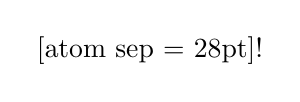
\begin{tikzpicture}
  \node (base) at (0,0) {};
  \chemHexagoneHaw[atom sep = 28pt] (-32pt,0pt)
  \node at (base) {\chemfig[atom sep = 28pt]{!\glucoseHaw}};
\end{tikzpicture}
\end{boiteCodeTex}
  \section{Lipides}

%%
\subsection{Acide gras}
  
\begin{boiteCodeTex}{}
  \chemfig{!\palmitique} \\[8pt]
  \chemfig{!\linoleique}
  \chemfig{!\linolenique} \\[8pt]
  \chemfig{!\oleique}
  \chemfig{!\arachidonique} \\[8pt]
  \chemfig{!\eicosaPentaenoique}
  \chemfig{!\docosaHexanoique}
\end{boiteCodeTex}

\begin{boiteCodeTex}{}
  \chemfig{!\steraiqueSemiDev}
  \chemfig{!\oleiqueSemiDev}
  \chemfig{!\oleateSemiDev}
  \chemfig{!\caproiqueSemiDev}
\end{boiteCodeTex}
  
%%  
\subsection{Triglycérides et phospholipides}

\begin{boiteCodeTex}{}
  \chemfig{!\palmitine} \\
  \chemfig[atom sep = 14pt]{[:60]!\oleine}
  \chemfig[atom sep = 14pt]{!\arachidonine}
\end{boiteCodeTex}
  
\begin{boiteCodeTex}{}
  \chemfig{!\oleineSemiDev}
  \chemfig{!\palmitineSemiDev}
  \chemfig{!\caproineSemiDev}
\end{boiteCodeTex}

\begin{boiteCodeTex}{}
  \chemfig{!\phosphatidylcholine}
\end{boiteCodeTex}

%%
\subsection{glycérol et stérols}

\begin{boiteCodeTex}{}
  \chemfig{!\glycerol} \qq{}
  \chemfig{!\glycerolSemiDev}
\end{boiteCodeTex}
  
\begin{boiteCodeTex}{}
  \chemfig{!\cholesterol}
\end{boiteCodeTex}

%%
\subsection{Sous-molécules utiles}
  
\subsubsection{Pour les chaînes dans les triglycérides}

\begin{boiteCodeTex}{}
  \chemfig{[:-30] !\tricaproique}
  \chemfig{[:-30] !\trilaurique} \\
  \chemfig{[:-30] !\tripalmitique}
  \chemfig{[:-30] !\trioleique} \\
  \chemfig{[:-30] !\trilinoleique}
  \chemfig{[:-30] !\trilinolenique} \\
  \chemfig{[:-30] !\trieicosapenta}
  \chemfig{[:-30] !\triarachidonique}
  \chemfig{[:-30] !\tridocosahexa}
\end{boiteCodeTex}
  
\subsubsection{Pour les triglycérides}

\begin{boiteCodeTex}{}
  \chemfig[atom sep = 18pt]{A-[:30] !\glycero{!\lh B} !\lb C }
  \chemfig[atom sep = 18pt]{[:60] !\triester{A}{B}{C}}
  \chemfig[atom sep = 18pt]{!\triesterSat{A}{B}C} \\
  \chemfig[atom sep = 14pt]{!\triester {!\trioleique} {!\tricaproique} {!\trilinolenique}}
  \chemfig[atom sep = 14pt]{!\triesterSat {!\lb !\trioleique} {!\tripalmitique} !\lb !\trilaurique}
\end{boiteCodeTex}

  \section{Glucides}

%%
\subsection{Amidon}

\begin{boiteCodeTex}{}
  \chemfig{!\amylopectineHaw}
\end{boiteCodeTex}

%%
\subsection{Glucose et fructose}

\begin{boiteCodeTex}{}
  \chemfig{!\glucoseHaw}
  \chemfig{!\glucoseCycle} \\
  \chemfig{!\glucose} \\[8pt]
  \chemfig{!\glucoseSemiDev}
\end{boiteCodeTex}

\begin{boiteCodeTex}{}
  \chemfig{!\fructoseHaw}
  \chemfig{!\fructofuranoseHaw}
  \chemfig{!\fructoseCycle} \\
  \chemfig{!\fructose} \\[8pt]
  \chemfig{!\fructoseSemiDev}
\end{boiteCodeTex}

%%
\subsection{Galactose et saccharose}

\begin{boiteCodeTex}{}
  \chemfig{!\galactoseHaw}
  \chemfig{!\saccharoseHaw}
\end{boiteCodeTex}

%%
\subsection{Ribose et desoxyribose}

\begin{boiteCodeTex}{}
  \chemfig{A !\ribose B}
  \chemfig{A !\desoxyribose B}
  \chemfig{A !\riboseHaw B}
  \chemfig{A !\desoxyriboseHaw B}
\end{boiteCodeTex}

  \section{Acides alpha aminés et protéines}

%%
\subsection{Formules topologiques}

\begin{boiteCodeTex}{}
  \chemfig{!\arginine}
  \chemfig{!\histidine}
  \chemfig{!\lysine}
  \chemfig{!\aspartique}
\end{boiteCodeTex}
  
\begin{boiteCodeTex}{}
  \chemfig{!\glutamique}
  \chemfig{!\serine}
  \chemfig{!\threonine}
  \chemfig{!\asparagine}
\end{boiteCodeTex}
  
\begin{boiteCodeTex}{}
  \chemfig{!\glutamine}
  \chemfig{!\cysteine}
  \chemfig{!\selenocysteine}
  \chemfig{!\glycine}
\end{boiteCodeTex}
  
\begin{boiteCodeTex}{}
  \chemfig{!\proline}
  \chemfig{!\alanine}
  \chemfig{!\valine}
  \chemfig{!\isoleucine}
  \chemfig{!\leucine}
\end{boiteCodeTex}
  
\begin{boiteCodeTex}{}
  \chemfig{!\methionine}
  \chemfig{!\phenylalanine}
  \chemfig{!\tyrosine}
  \chemfig{!\tryptophane}
\end{boiteCodeTex}

%%
\subsection{Formules semi-développées, représentation de Fischer et de Cram}

\begin{boiteCodeTex}{}
  \chemfig{!\alanineSemiDev} \qq{}
  \chemfig{!\asparagineSemiDev} \qq{}
  \chemfig{!\glycineSemiDev} \\[8pt]
  \chemfig{!\cysteineSemiDev} \\[8pt]
\end{boiteCodeTex}

\begin{boiteCodeTex}{}
  \chemfig{!\alanineL} \quad
  \chemfig{!\alanineD} \quad
  \chemfig{!\valineL} \quad
  \chemfig{!\valineD}
\end{boiteCodeTex}

%%
\subsection{Polypeptides et groupements prosthétiques}

\begin{boiteCodeTex}{}
  \chemfig{ [:-30] H_2N !\alanineH !\HN !\glycineB !\NH !\cysteineH !\HN !\isoleucineB !\NH !\valineH OH }
\end{boiteCodeTex}

\begin{boiteCodeTex}{}
  \chemfig[atom sep = 18pt]{!\hemeB}
\end{boiteCodeTex}

  \section{Vitamines}

\subsection{Vitamines B et C}

\begin{boiteCodeTex}{}
  \chemfig{!\thiamine}               % B1
  \chemfig{!\riboflavine} \\         % B2
  \chemfig{!\nicotinamide} \qq{}     % B3
  \chemfig{!\acideNicotinique} \qq{} % B3
  \chemfig{!\acidePantothenique}     % B5
\end{boiteCodeTex}{}

\begin{boiteCodeTex}{}
  \chemfig{!\pyroxidine}   % B6
  \chemfig{!\biotine} \\   % B8
  \chemfig[atom sep = 18pt]{!\acideFolique} % B9
\end{boiteCodeTex}

\begin{boiteCodeTex}{}
  \chemfig[atom sep = 18pt]{!\cyanocobalamine} % B12
\end{boiteCodeTex}

\begin{boiteCodeTex}{}
  \chemfig{!\acideAscorbique} % C
\end{boiteCodeTex}

\subsection{Vitamines A, D, E, K$_1$ et K$_2$}

\begin{boiteCodeTex}{}
  \chemfig[atom sep = 18pt]{!\retinol} \\      % A
  \chemfig[atom sep = 18pt]{!\cholecarciferol} % D
\end{boiteCodeTex}
  
\begin{boiteCodeTex}{}
  \chemfig[atom sep = 18pt]{!\tocopherol} \\[8pt] % E
  \chemfig[atom sep = 18pt]{!\tocotrienol}        % E
\end{boiteCodeTex}
  
\begin{boiteCodeTex}{}
  \chemfig[atom sep = 18pt]{!\phylloquinone} \\[8pt] % K1
  \chemfig[atom sep = 18pt]{!\menatetrenone}         % K2
\end{boiteCodeTex}

  \section{Hormones}

\begin{boiteCodeTex}{}
  \chemfig{!\creatinine}
  \chemfig{!\DOPA}
  \chemfig{!\DOPAH} \\[8pt]
  \chemfig{!\prostaglandine}
\end{boiteCodeTex}

%%
\subsection{Corticoïdes et minéralocorticoïdes}

\begin{boiteCodeTex}{}
  \chemfig{!\cortisol} \hspace*{-50pt}
  \chemfig{!\corticosterone} \hspace*{-64pt}
  \chemfig{!\aldosterone}
\end{boiteCodeTex}

%%
\subsection{Oestrogènes}

\begin{boiteCodeTex}{}
  \chemfig{!\estrone} \hspace*{-40pt}
  \chemfig{!\estriol} \hspace*{-56pt}
  \chemfig{!\estradiol}
\end{boiteCodeTex}

%%
\subsection{Androgènes}

\begin{boiteCodeTex}{}
  \chemfig{!\testosterone} \hspace*{-12pt}
  \chemfig{!\dihydrotestosterone} \hspace*{-12pt}
  \chemfig{!\androstenedione}
\end{boiteCodeTex}

\begin{boiteCodeTex}{}
  \chemfig{!\DHEA}
  \chemfig{!\DHEAS}
\end{boiteCodeTex}

%%
\subsection{Progestatives}

\begin{boiteCodeTex}{}
  \chemfig{!\progesterone}
\end{boiteCodeTex}

  \section{Nucléotides}

\subsection{Bases nucléiques}

\begin{boiteCodeTex}{}
  \chemfig{A- !\adenine} \hspace*{-20pt}
  \chemfig{A- !\cytosine}
  \chemfig{A- !\guanine} \hspace*{-20pt}
  \chemfig{A- !\thymine} 
  \chemfig{A- !\uracile} 
\end{boiteCodeTex}

%%
\subsection{Ribonucléosides et désoxyribonucléosides}

\begin{boiteCodeTex}{}
  \chemfig{!\adenosine}
  \chemfig{!\cytidine} 
  \chemfig{!\guanosine} \\[8pt]
  \chemfig{!\thymidine}
  \chemfig{!\uridine}  
\end{boiteCodeTex}

\begin{boiteCodeTex}{}
  \chemfig{!\adenosineHaw}
  \chemfig{!\cytidineHaw} 
  \chemfig{!\guanosineHaw} \\[8pt]
  \chemfig{!\thymidineHaw}
  \chemfig{!\uridineHaw}  
\end{boiteCodeTex}

\begin{boiteCodeTex}{}
  \chemfig{!\desoxyAdenosineHaw}
  \chemfig{!\desoxyCytidineHaw} 
  \chemfig{!\desoxyGuanosineHaw} \\[8pt]
  \chemfig{!\desoxyThymidineHaw}
  \chemfig{!\desoxyUridineHaw}  
\end{boiteCodeTex}

%%
\subsection{Adénosine triphosphate et diphosphate}
\begin{boiteCodeTex}{}
  \chemfig{!\ADP}
  \chemfig{!\ATP}
\end{boiteCodeTex}

\begin{boiteCodeTex}{}
  \chemfig{!\ADPHaw}
  \chemfig{!\ATPHaw}
\end{boiteCodeTex}

  \section{Médicaments et produits de synthèse}

\subsection{Aspirine}

\begin{boiteCodeTex}{}
  \chemfig{!\aspirineSemiDev}
  \chemfig{!\aspirine} \qq{}
  \chemfig{!\acideSalicylique}
\end{boiteCodeTex}
  
\subsection{Paracétamol}

\begin{boiteCodeTex}{}
  \chemfig{!\paracetamol}
  \chemfig{!\paracetamolSemiDev}
  \chemfig{!\paracetamolDev}
\end{boiteCodeTex}

\subsection{Aspartame}

\begin{boiteCodeTex}{}
  \chemfig{!\aspartame}
  \chemfig{[:-30]H_2N !\aspartiqueH !\NH !\phenylalanineB OH}
\end{boiteCodeTex}
  
\subsection{Divers}

\begin{boiteCodeTex}{}
  \chemfig{!\bisphenolA} \qq{}
  \chemfig{!\bisphenolASemiDev}
\end{boiteCodeTex}

  \section{Molécules odorantes}

\begin{boiteCodeTex}{}
  \chemfig{!\geraniol} \quad
  \chemfig{!\geraniolSemiDev} \quad
  \chemfig{!\vanilline} \quad
  \chemfig{!\ethylvanilline}
\end{boiteCodeTex}

\begin{boiteCodeTex}{}
  \chemfig{!\oxyphenylone} \quad
  \chemfig{!\limonene} \quad
  \chemfig{!\limoneneSemiDev} \quad
  \chemfig{!\acetateIsoamyle}
\end{boiteCodeTex}

  \input{biomolecules-doc-divers}
\end{document}
